\documentclass{beamer}
\usetheme{Berkeley}
\usecolortheme{whale}
\title{Anttris -- CSE 326}
\author{%
\and Chris Aikman
\and Benji Cope
\and Skyler Manzanares
\and Hugo Rivera
\and Sean Turner}
\date{April 27, 2015}

\graphicspath{{pngs/}}

\begin{document}

\begin{frame}
\titlepage
\end{frame}

\begin{frame}
    \frametitle{Example frame}
    Items go!
\begin{itemize}
\pause \item A!
\pause \item B!
\pause \item C!
\end{itemize}

\begin{alertblock}{Solution}
Solved!
\end{alertblock}

\end{frame}

\section{Paper Summary}
\begin{frame}
    These pics don't work.
\includegraphics[width=0.4\linewidth]{yellow_bands.png}
\pause
\includegraphics[width=0.5\linewidth]{many_layouts.png}
\end{frame}


%%%% Stuff from Shin's slides

%% moved to relevant places

%%%% actual presentation


\section{Project}

%% from Shin's slides
\begin{frame}
  \frametitle{Motivation} % 
\end{frame}

\begin{frame}
  \frametitle{Objective} % SKYLER: rub it in
\end{frame}

%% ----- %%

\begin{frame}
    \frametitle{GUI} % CHRIS
    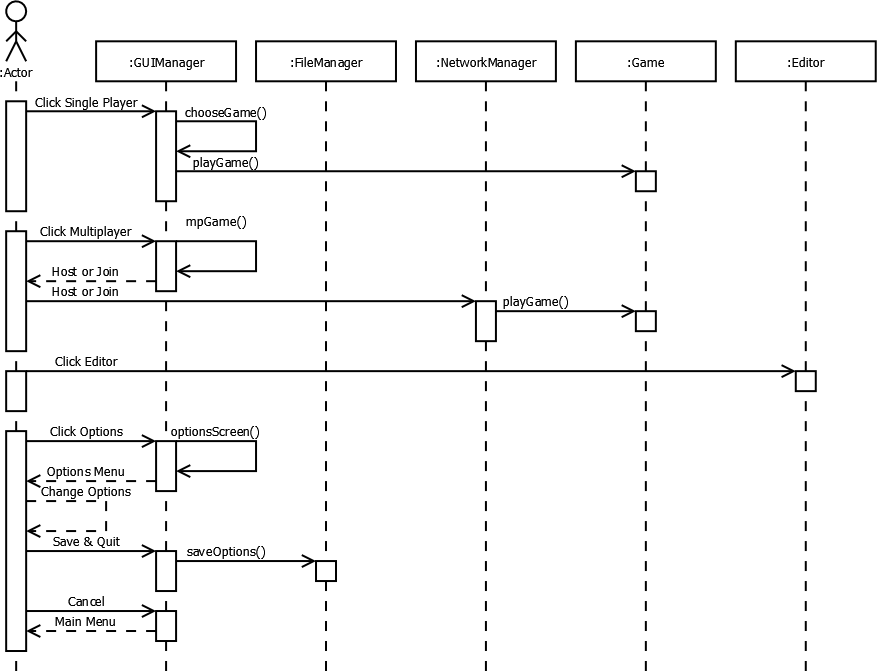
\includegraphics[width=1\linewidth]{Anttris_GUISequence.png}
\end{frame}

\begin{frame}
    \frametitle{GUI} % CHRIS
    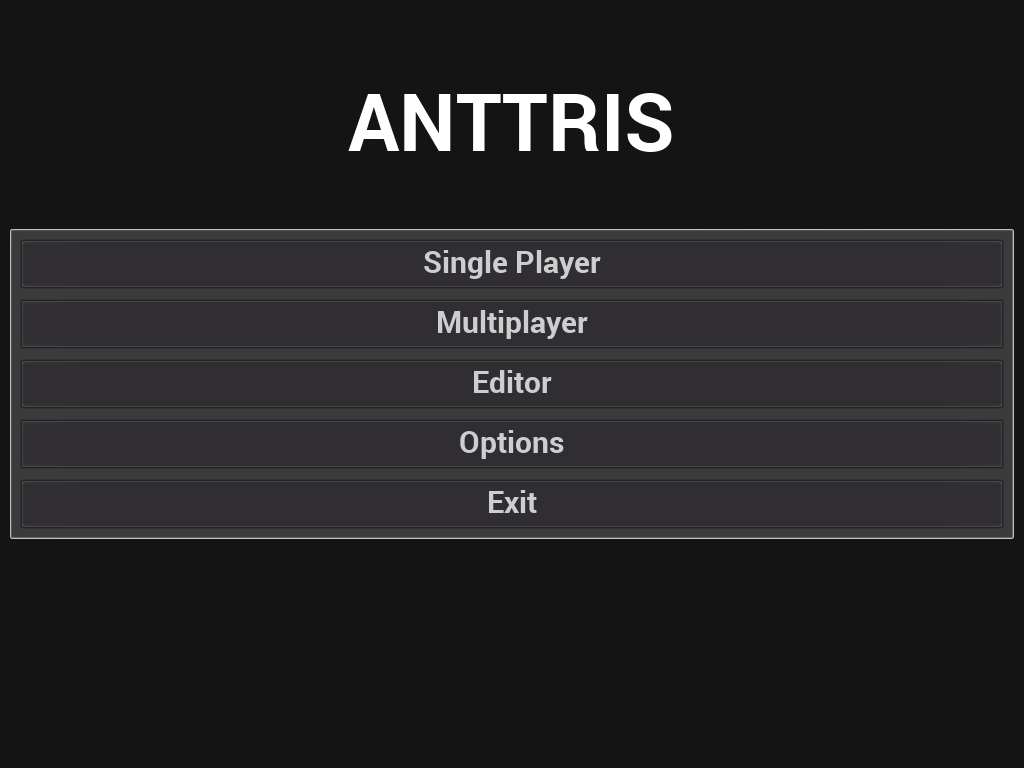
\includegraphics[width=1\linewidth]{Anttris_MainMenu.png}
\end{frame}

\begin{frame}
    \frametitle{Data Manager} % CHRIS
    \begin{itemize}
	\item Serialize Data
	\pause \item Save / Load Options
	\pause \item Save / Load Puzzles
	\end{itemize}
\end{frame}

\begin{frame}
    \frametitle{Editor} % HUGO
\end{frame}

\begin{frame}
    \frametitle{Generator, Solver} % CHRIS
\end{frame}

\begin{frame}
    \frametitle{Networking} % SKYLER
    \begin{itemize}
        \pause \item Multiplayer
        \pause \item P2P
        \begin{itemize}
            \pause \item Non-random Opponents
            \pause \item Network Information
        \end{itemize}
        \pause \item Key Events
            \pause \item Start of Game
            \pause \item Transform Puzzle
            \pause \item Select Blocks
            \pause \item Game End
\end{frame}

\begin{frame}
    \frametitle{Rules} % CHRIS
\end{frame}

\begin{frame}
    \frametitle{Grand Summary} % BENJI
\end{frame}


\section{Implementation}
\begin{frame}
  \frametitle{Approach} % Hugo? idk
\end{frame}

\begin{frame}
    \frametitle{Godot} % HUGO
\end{frame}

\begin{frame}
    \frametitle{GD Script} % HUGO 
\end{frame}

\begin{frame}
    \frametitle{Code Overview} % line counts..., UML
\end{frame}


\section{Workflow} % SEAN
\begin{frame}
    \frametitle{Our Workflow} 
    \begin{itemize}
    		\pause \item We used Github as our source control.
    		\pause \item To facilitate an agile workflow we used Zenhub.
    		\begin{itemize}
    		\pause \item Zenhub integrates a Scrum board right in Github.
    		\pause \item We set out to use certain parts of Scrum, but we're students!
    		\pause \item Which means, we didn't always adhere to the rules.
    		\end{itemize}
    		\pause \item Continuous Integration
    		\begin{itemize}
    			\pause \item Travis CI. It's awesome and everyone should try it!
    			\pause \item Not to mention free for open source projects. 
    		\end{itemize}
    		\pause \item Branches
    		\begin{itemize}
    			\pause \item We used branches and pull requests to merge changes.
    			\pause \item This facilites easy code reviews before things get broken!
    		\end{itemize}
    \end{itemize}
\end{frame}

\begin{frame}
    \frametitle{Workflow, Continued}
    \begin{itemize}
    		\pause \item Unit testing
    		\begin{itemize}
    			\pause \item We used the [G]odot [U]nit [T]esting framework, aka GUT.
    			\pause \item This works nicely with Travis, thanks to a Python script Hugo wrote to catch return values and report on unit test results.
    			\pause \item This project is hosted on Bitbucket at {\url https://bitbucket.org/bitwes/gut/overview}.
    		\end{itemize}
	\end{itemize}     
\end{frame}

\begin{frame}
    \frametitle{Project Pace} % BENJI
\end{frame}

\begin{frame}
  \frametitle{What we learned} % SKYLER
\end{frame}

%% From Dr Shin's slides
\begin{frame}
  \frametitle{Demo} % ALL, BRING ANDROIDS, LAPTOPS (OSX, WINDOWS, LINUX)
\end{frame}
%% ------ %%



\end{document}
